\documentclass{beamer}

\mode<presentation> {

% The Beamer class comes with a number of default slide themes
% which change the colors and layouts of slides. Below this is a list
% of all the themes, uncomment each in turn to see what they look like.

%\usetheme{default}
%\usetheme{AnnArbor}
%\usetheme{Antibes}
%\usetheme{Bergen}
%\usetheme{Berkeley}
%\usetheme{Berlin}
%\usetheme{Boadilla}
%\usetheme{CambridgeUS}
%\usetheme{Copenhagen}
%\usetheme{Darmstadt}
%\usetheme{Dresden}
%\usetheme{Frankfurt}
%\usetheme{Goettingen}
%\usetheme{Hannover}
%\usetheme{Ilmenau}
%\usetheme{JuanLesPins}
%\usetheme{Luebeck}
\usetheme{Madrid}
%\usetheme{Malmoe}
%\usetheme{Marburg}
%\usetheme{Montpellier}
%\usetheme{PaloAlto}
%\usetheme{Pittsburgh}
%\usetheme{Rochester}
%\usetheme{Singapore}
%\usetheme{Szeged}
%\usetheme{Warsaw}

% As well as themes, the Beamer class has a number of color themes
% for any slide theme. Uncomment each of these in turn to see how it
% changes the colors of your current slide theme.

%\usecolortheme{albatross}
%\usecolortheme{beaver}
%\usecolortheme{beetle}
%\usecolortheme{crane}
%\usecolortheme{dolphin}
%\usecolortheme{dove}
%\usecolortheme{fly}
%\usecolortheme{lily}
%\usecolortheme{orchid}
%\usecolortheme{rose}
%\usecolortheme{seagull}
%\usecolortheme{seahorse}
%\usecolortheme{whale}
%\usecolortheme{wolverine}

%\setbeamertemplate{footline} % To remove the footer line in all slides uncomment this line
%\setbeamertemplate{footline}[page number] % To replace the footer line in all slides with a simple slide count uncomment this line

%\setbeamertemplate{navigation symbols}{} % To remove the navigation symbols from the bottom of all slides uncomment this line
}

%% Make top right box blank for each new frame
\usepackage{tikz}
\usepackage{listings}
\lstset{language=SQL,morekeywords={PREFIX,java,rdf,rdfs,url}}
\usepackage{graphicx} % Allows including images
\usepackage{booktabs} % Allows the use of \toprule, \midrule and \bottomrule in tables
\usepackage[utf8]{inputenc}

\newcommand{\infoForRightCorner}[1]{%
\tikz[remember picture,overlay]{
    \node[anchor=north east, text=white] at (current page.north east) {#1};}
    }

%----------------------------------------------------------------------------------------
%	TITLE PAGE
%----------------------------------------------------------------------------------------

\title[Google Home]{Google Home Final Presentation} % The short title appears at the bottom of every slide, the full title is only on the title page

\author{Mehmet Kardan, Hanna Köb, Mathias Meinschad, Daniel Linter} % Your name
\institute[UCLA] % Your institution as it will appear on the bottom of every slide, may be shorthand to save space
{
University of Innsbruck - STI \\ % Your institution for the title page
}
\date{June 24, 2020} % Date, can be changed to a custom date

\begin{document}

\begin{frame}
\titlepage % Print the title page as the first slide
\end{frame}

\begin{frame}
\small
\frametitle{Agenda} % Table of contents slide, comment this block out to remove it
\infoForRightCorner{Daniel Linter}
\tableofcontents % Throughout your presentation, if you choose to use \section{} and \subsection{} commands, these will automatically be printed on this slide as an overview of your presentation
\end{frame}

%----------------------------------------------------------------------------------------
%	PRESENTATION SLIDES
%----------------------------------------------------------------------------------------

%------------------------------------------------
\section{Introduction to Google Home}

\begin{frame}
\frametitle{Introduction to Google Home}
\infoForRightCorner{Daniel Linter}
\begin{center}

\includegraphics[scale=0.35]{pictures/google-home.png} 
\end{center}
\begin{itemize}
\item Founded by Google in 2016
\item Development through Googles developer console and Dialogflow
\item Creating skills pretty easy
\item No programming skills required
\end{itemize}
\end{frame}

\subsection{Device Types \& Traits}

\begin{frame}
\frametitle{Device Types \& Traits}
\infoForRightCorner{Daniel Linter}
\begin{center}
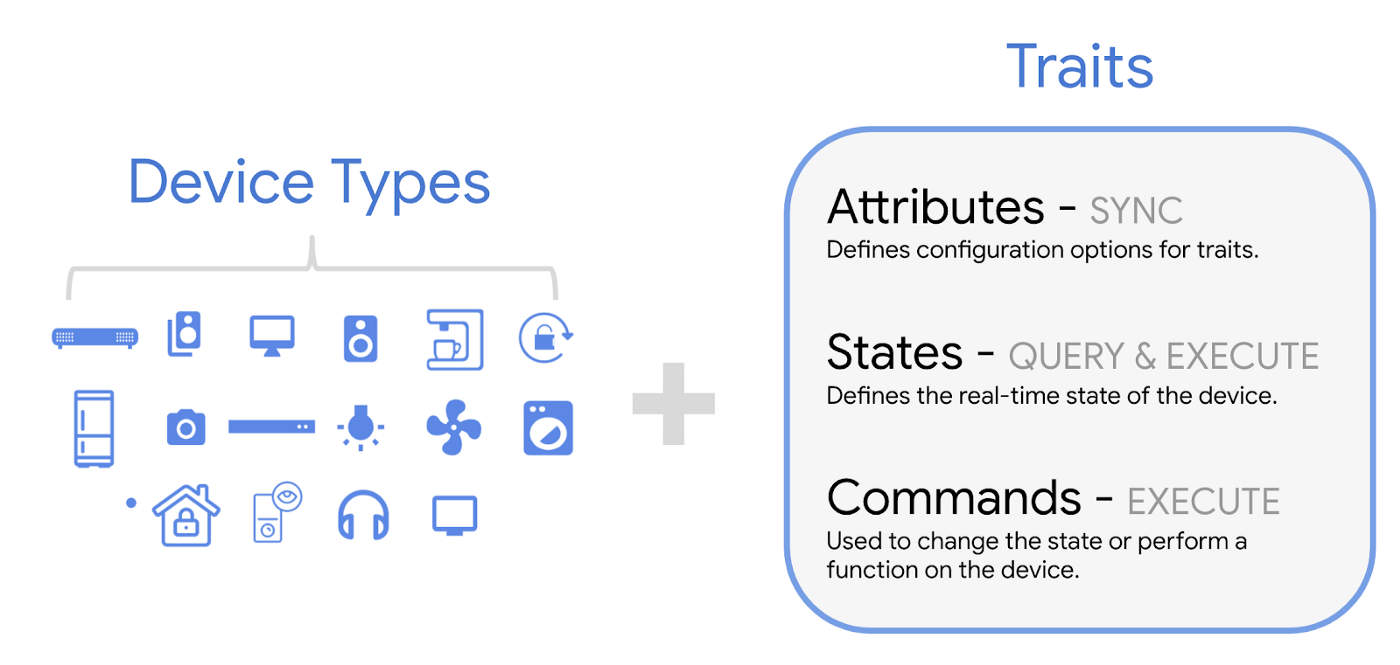
\includegraphics[scale=0.2]{pictures/state_commands.png} 
\end{center}
\begin{itemize}
\item Various device types ( air purifier to yogurt maker )
\item Capabilities of a device $\Rightarrow$ traits
\end{itemize}
\end{frame}

%------------------------------------------------

\subsection{Execution Path}

\begin{frame}
\frametitle{Execution Path}
\infoForRightCorner{Daniel Linter}
\begin{center}
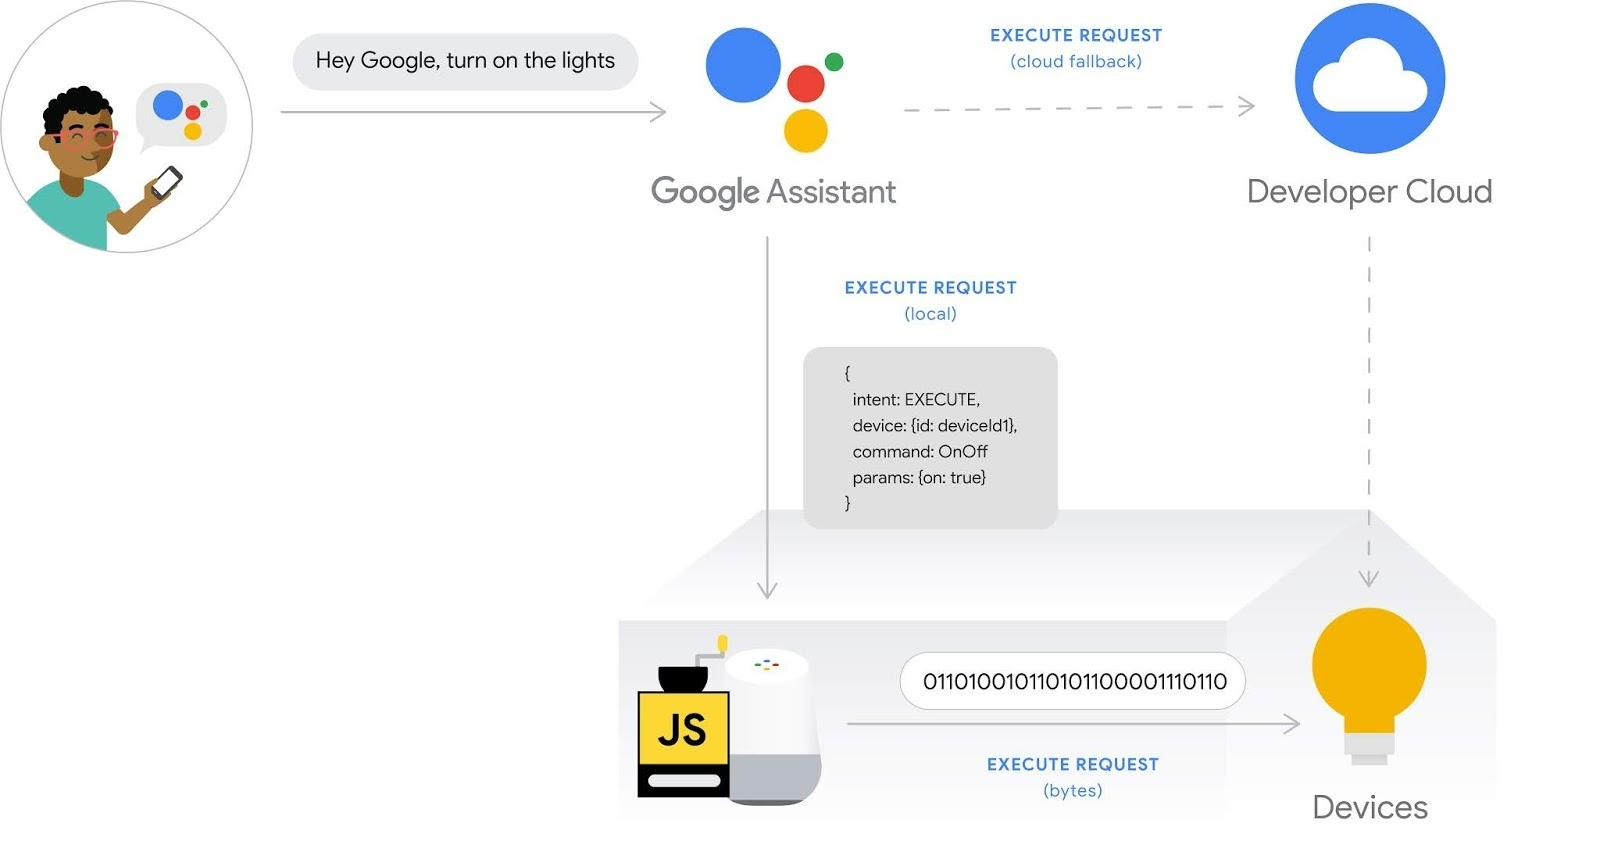
\includegraphics[scale=0.2]{pictures/execution-path.png}
\end{center}
\end{frame}

%------------------------------------------------

\section{Introduction to Dialogflow}

\begin{frame}
\infoForRightCorner{Daniel Linter}
\frametitle{Introduction to Dialogflow}
\begin{center}
\begin{itemize}
\item Service developed and provided by Google
\item Natural language tool to create conversational user interfaces for apps, chatbots, etc.
\item By adding 'Training phrases' Dialogflow automatically trains the machine learning model
\end{itemize}
\end{center}
\end{frame}

\subsection{Intents}

\begin{frame}
\frametitle{Intents}
\infoForRightCorner{Hanna Köb}
\begin{center}
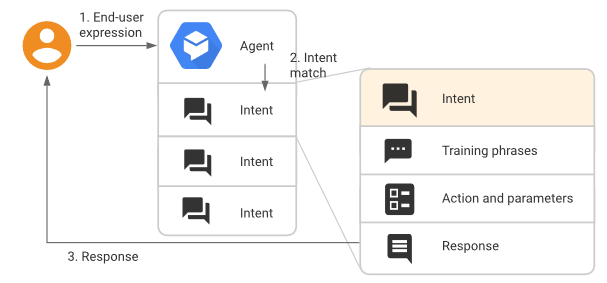
\includegraphics[width=0.8\textwidth]{pictures/intent.png}

\end{center}
\end{frame}

%------------------------------------------------

\subsection{Entities}

\begin{frame}
\frametitle{Entities}
\infoForRightCorner{Hanna Köb}
\begin{center}
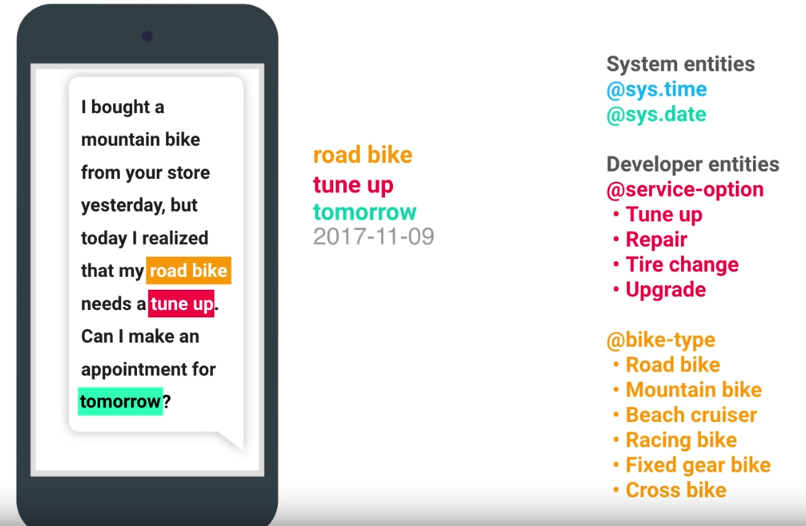
\includegraphics[width=0.8\textwidth]{pictures/entities2.png}
\end{center}
\end{frame}

%------------------------------------------------

\subsection{Architecture}

\begin{frame}
\frametitle{Architecture}
\infoForRightCorner{Hanna Köb}
\begin{center}
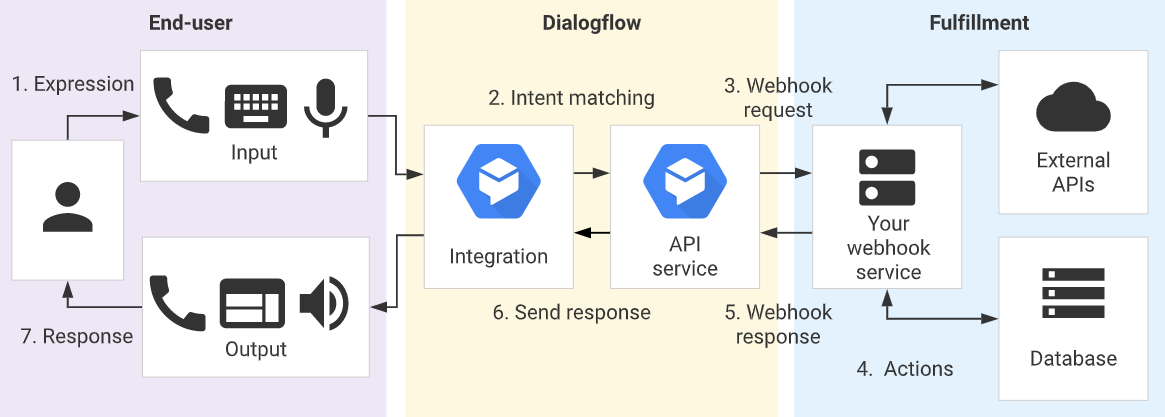
\includegraphics[width=\textwidth]{pictures/fulfillment_flow.png} 
\end{center}
\end{frame}

\section{Implementation}

\begin{frame}
\frametitle{Implementation}
\infoForRightCorner{Hanna Köb}
\begin{itemize}
\item Coding in JavaScript
\end{itemize}
\begin{center}
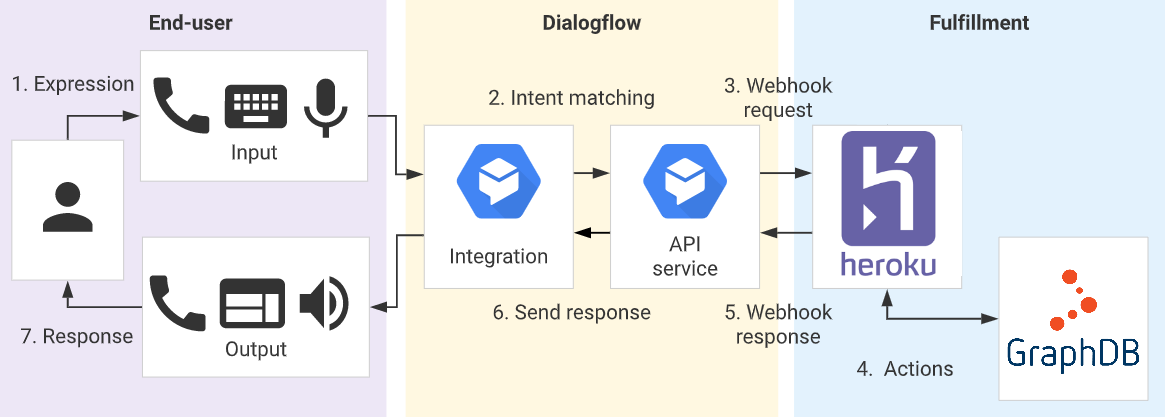
\includegraphics[width=\textwidth]{pictures/fulfillment_flow2.png} 
\end{center}
\end{frame}

%------------------------------------------------

\subsection{Entities Extraction}
\begin{frame}[fragile]
\frametitle{Entities Extraction}
\infoForRightCorner{Hanna Köb}
\begin{itemize}
\item An entity for each class in the knowledge graph is created
\begin{lstlisting}[basicstyle=\ttfamily,frame=single]
SELECT DISTINCT ?class
WHERE {
	?s a ?class .
}
\end{lstlisting}
\item Then schema.org's property \textit{name} is used to fill the entities with values
\begin{lstlisting}[basicstyle=\ttfamily,frame=single]
PREFIX sc: <http://schema.org/> 
SELECT ?name 
WHERE { 
	?resource  a [entityTypeName] . 
	?resource sc:name ?name . 
}	
\end{lstlisting}
\end{itemize}
\end{frame}

\begin{frame}[fragile]
\frametitle{Entities Extraction cont'd}
\infoForRightCorner{Hanna Köb}

\begin{center}
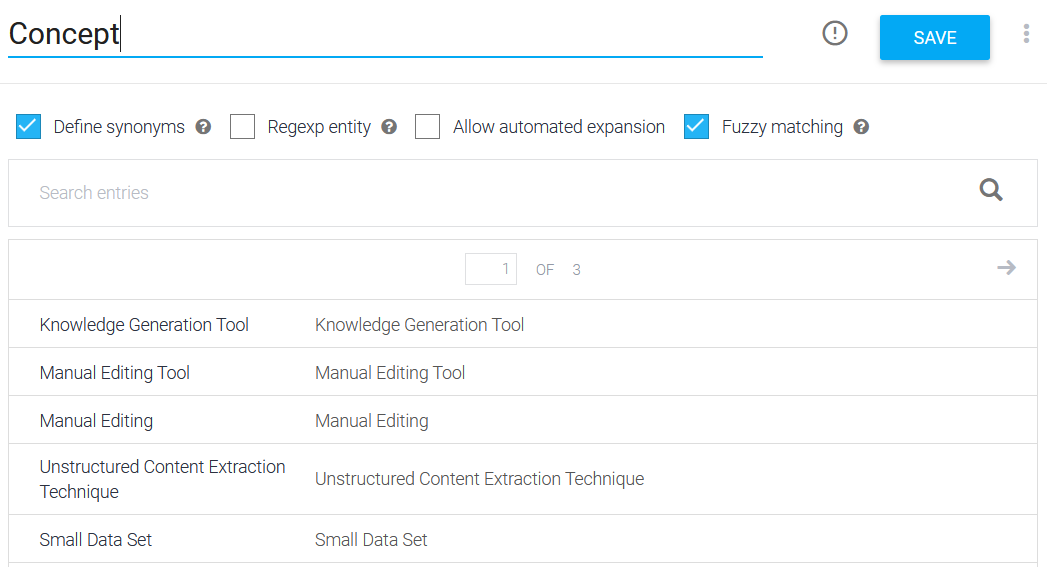
\includegraphics[scale=0.5]{pictures/dialogflow_entities.png}
\end{center}

\end{frame}

%------------------------------------------------

\section{Queries, Intents and Response Handling}
\begin{frame}
\frametitle{Queries, Intents and Response Handling}
\infoForRightCorner{Mehmet Kardan}
\begin{itemize}
\item Divided questions into the Intents.
\item Defined a query for specific intent type.
\item Response handling function for the queries.
\end{itemize}
\end{frame}

%------------------------------------------------
\subsection{Intents}

\begin{frame}
\frametitle{Intents}
\infoForRightCorner{Mehmet Kardan}
\begin{itemize}
\item 6 question types defined in Dialogflow
\begin{itemize}
\item Difference Type Question
\item Example Type Questions
\item List Type Questions
\item Narrower Type Question
\item Step Type Questions
\item What is Type Questions
\end{itemize}
\end{itemize}
\end{frame}

%------------------------------------------------
\subsection{Queries}

\begin{frame}
\frametitle{Queries}
\infoForRightCorner{Mehmet Kardan}
\begin{itemize}
\item Queries are encoded with Query String module.
\item For each intent type, we defined the following queries.
\end{itemize}
\end{frame}

%------------------------------------------------


\begin{frame}
\frametitle{Query for "What is Type Question"}
\infoForRightCorner{Mehmet Kardan}
\begin{center}
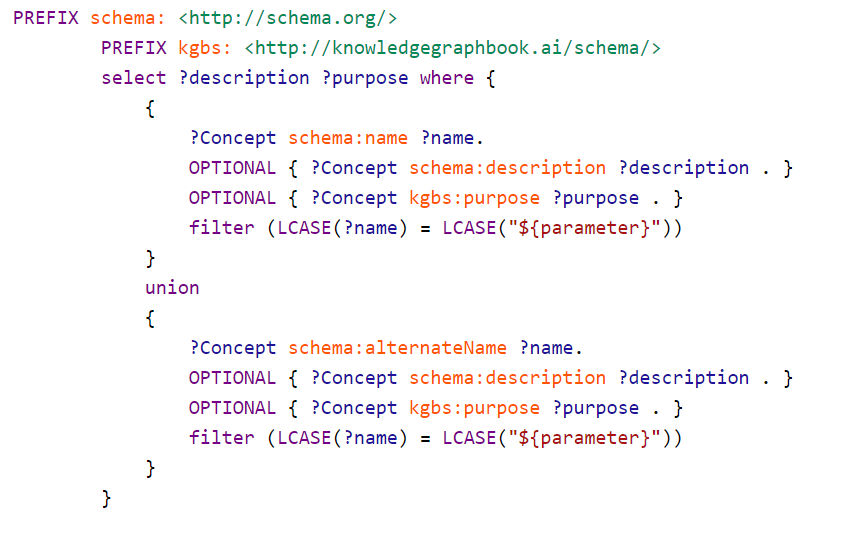
\includegraphics[scale=0.50]{pictures/what_is_type_query.png}
\end{center}
\end{frame}

\begin{frame}
\frametitle{Query for "Difference Type Questions"}
\infoForRightCorner{Mehmet Kardan}
\begin{center}
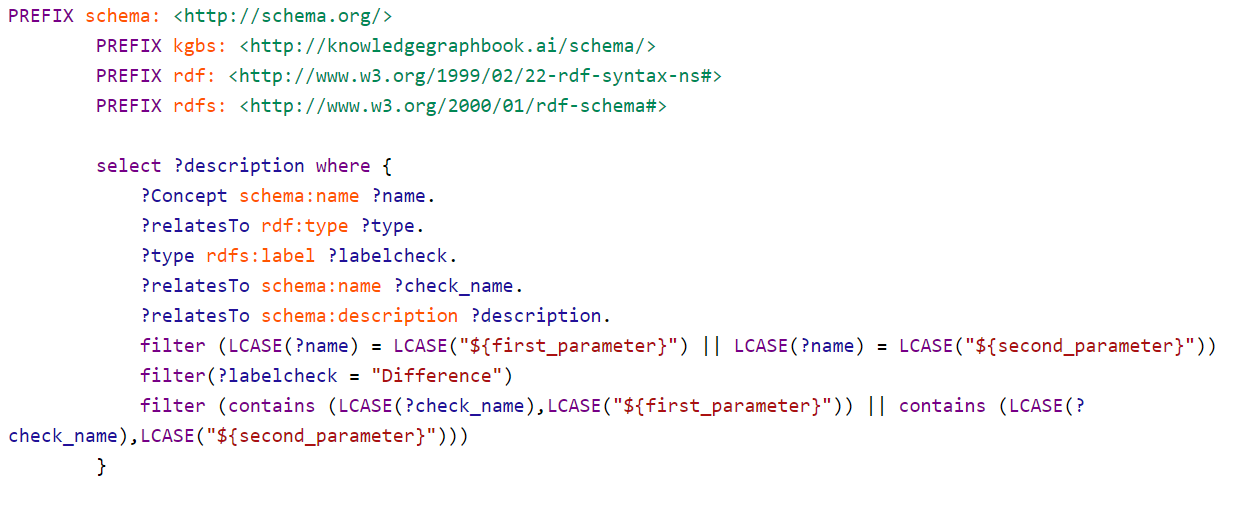
\includegraphics[scale=0.45]{pictures/difference_type_query.png}
\end{center}
\end{frame}

\begin{frame}
\frametitle{Query for "List Type Questions"}
\infoForRightCorner{Mehmet Kardan}
\begin{center}
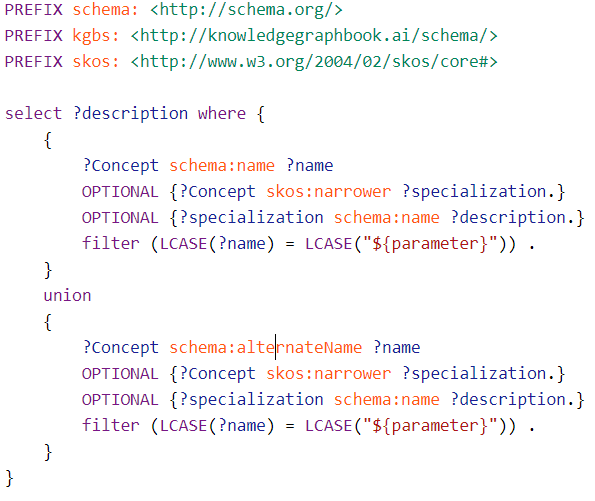
\includegraphics[scale=0.5]{pictures/list_type_query.png}
\end{center}
\end{frame}

\begin{frame}
\frametitle{Query for "Example Type Questions"}
\infoForRightCorner{Mathias Meinschad}
\begin{center}
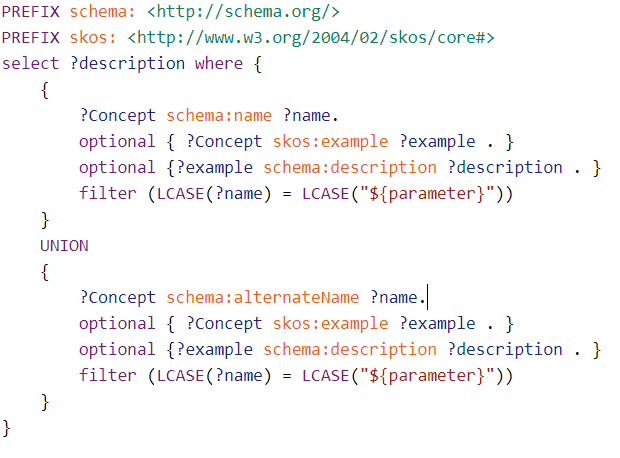
\includegraphics[scale=0.5]{pictures/example_type_query.png}
\end{center}
\end{frame}

\begin{frame}
\frametitle{Query for "Step Type Questions"}
\infoForRightCorner{Mathias Meinschad}
\begin{center}
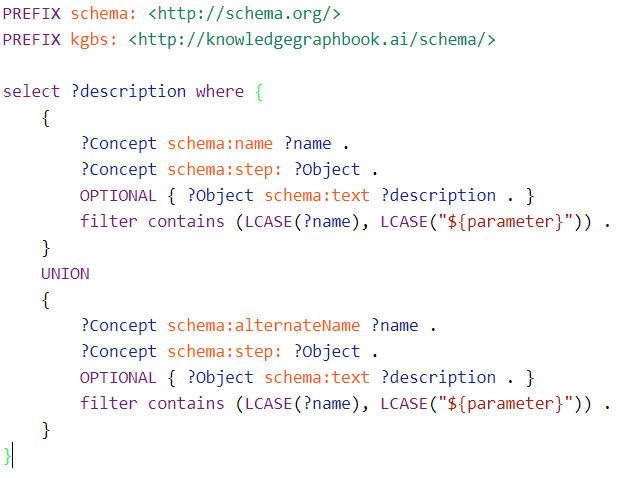
\includegraphics[scale=0.5]{pictures/step_type_query.png}
\end{center}
\end{frame}

\begin{frame}
\frametitle{Query for "Narrower Type Questions"}
\infoForRightCorner{Mathias Meinschad}
\begin{center}
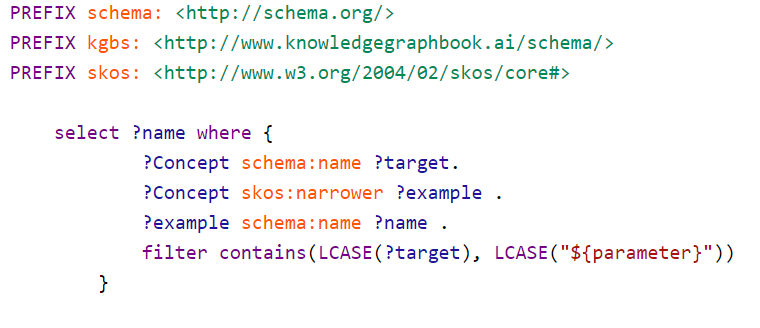
\includegraphics[scale=0.5]{pictures/narrower_type_query.png}
\end{center}
\end{frame}

\subsection{Response Handling}

\begin{frame}
\frametitle{Response Handling}
\infoForRightCorner{Mathias Meinschad}
\begin{center}
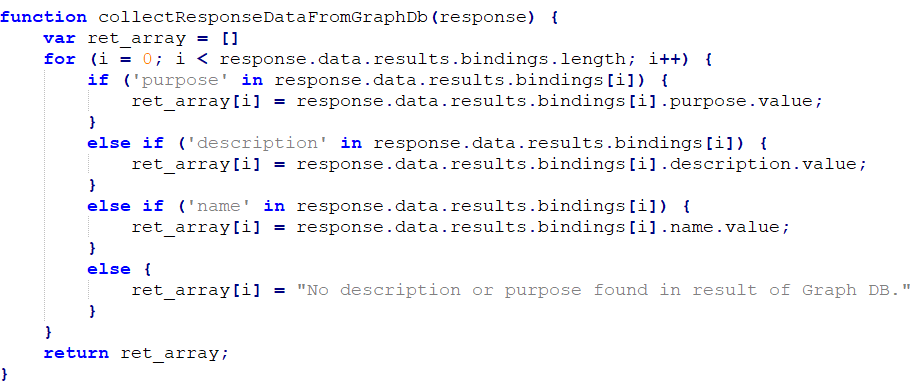
\includegraphics[scale=0.50]{pictures/response_handling.png} 
\end{center}
\begin{itemize}
\item 3 different types of response will be handled.
\item Default text for error handling.
\end{itemize}
\end{frame}

%------------------------------------------------

\section{Problems}

\begin{frame}
\frametitle{Problems}
\infoForRightCorner{Mathias Meinschad}
\begin{itemize}
\item Changing namespaces of GraphDB
\item No JavaScript library for GraphDB with authentication
\end{itemize}
\end{frame}

%------------------------------------------------


\section{Live Demo}

\begin{frame}
\frametitle{Live Demo}
\infoForRightCorner{Mathias Meinschad}
\begin{center}
{\fontsize{30}{40}\selectfont Live Demo}
\end{center}
\end{frame}

%------------------------------------------------

\begin{frame}
\begin{center}
{\fontsize{30}{40}\selectfont Thank you for your attention!}
\end{center}
\end{frame}

%------------------------------------------------

\end{document} 
